\documentclass[a4paper]{article}
\usepackage[labelfont={bf,it}, textfont=it, justification=centering]{caption}
\usepackage{titlesec}
\usepackage{amsmath}
\usepackage{amssymb}
\usepackage{bm}
\usepackage{graphicx}

\newcommand{\mat}[1]{\mathbf{#1}}
\renewcommand{\vec}[1]{\bm{#1}}

\setlength{\parindent}{0em}
\setlength{\parskip}{8pt}

\titlespacing\section{0pt}{12pt}{2pt}
\titlespacing\subsection{0pt}{12pt}{2pt}

\begin{document}
%\title{Sid's Group Report}
%\author{Siddhartha Menon}
%\date{\today}
%
%\maketitle

\section{Introduction to the Direct Method}
The direct method is possibly the most logically straightforward way to solve
for the values of the mesh points. It involves expressing the relationships of
the various grid points with each other through a system of simultaneous
equations, and then solving this system to obtain a vector containing the
solutions to the mesh points. Thus, in contrast to the iterative methods,
results are obtained at their final accuracy rather than being successively
improved over several cycles.

In our implementation we consider as system of the form:
\begin{align*}
	-4&V_1+V_2+0V_3+0V_4+V_5+\dots+0V_{16}&=0\\
	&V_1-4V_2+V_3+0V_4+0V_5+V_6+\dots+0V_{16}&=0\\
	&\vdots\\
	0&V_1+\dots+V_{12}+0V_{13}+0V_{14}+V_{15}-4V_{16}&=0\\
\end{align*}
Which can be expressed by the matrix equation:
\begin{equation}
	\mat{A}\vec{v}=\vec{b}
	\label{matEq}
\end{equation}
Where $\mat{A}$ is a matrix holding the coefficients of the system, $\vec{v}$
holds the voltage solutions, and $\vec{b}$ represents the right hand values of
the system. We could now apply a variety of generic matrix solving techniques
to find $\vec{v}$ but these methods quickly become impossible to practically
implement in larger problems for reasons discussed in the following sections.

\section{Implementation of the Direct Method}
The first thing to notice is that if we have a $N\times N$ grid then the
coefficient matrix has $N^4$ elements. This quartic growth means that the
storage space required quickly overtakes any realistic memory capacity.
Furthermore, even if one could procure such an expansive memory device, we
would still leave much to be desired in terms of efficiency. To understand why
this is, consider the structure of the matrix $\mat{A}$. We can notice that on
any given line there are at most five non zero elements: the point of interest,
and the four points around it. The rest of the elements on that row are
initialised to zero. The net effect of this is that the matrix $\mat{A}$ is
\emph{extremely} sparse, especially for large $N$. In fact the sparseness of
the matrix is the principle factor on which optimisations are made~\cite{NR}.
In the next section we discuss methods of storing large sparse matrices and the
challenges they present.

\subsection{Storage Systems for Sparse Matrices}
The essential idea behind sparse matrix compression is to minimise the required
storage space by only storing non-zero elements and there respective positions
such that all the information of the original matrix is still preserved.
Although there several compression schemes available~\cite{101matstore} we
utilised coordinate storage (COO) and compressed column storage (CCS).

The COO storage format is possibly the simplest to understand and implement. It
essentially involves storing three columns or arrays of data: one that tracks
the row numbers of the non-zero elements, another that tracks the column
numbers, and finally one that tracks the values themselves. While this method
offers a fairly good compression rate for large $N$ and is easy to implement,
it does suffer from a few drawbacks. Firstly, it does not optimise on the fact
that several non-zero elements share the same column (or row) number; secondly,
and more significantly, if we wanted to access the non-zero element $v$ with
row number $i$ and column number $j$ we would have to scan through all the
elements preceding it.

To overcome these shortfalls we may use the CCS format. As done previously we
will maintain three data sets, one of which will hold the non-zero values. The
second data set will hold the corresponding row values of those elements.
Finally, the third set holds holds \emph{column offsets} which tell us where in
the value set the next column begins. This not only reduces the space required
but also allows us to \emph{jump} to a requested value by referring to the
column offsets rather than scanning through every element~\cite{101matstore}.

\subsection{Formulating the Linear System}
The system of equations as described thus far holds no information with regard
to any specific geometry and therefore solves no particular problem. Thus, an
essential step is finding a mechanism where by the system can be tweaked to
reflect a given problem.

To see how this was achieved, consider the $4 \times 4$ grid shown
in Fig.~\ref{gridFig} with a voltage of 25V at $v_6$. How can this information
be represented in the system? The solution employed was to zero out the row
corresponding to $V_6$ (row 7 if we index from 0) and write a 1 into its
diagonal. We then write 25 in the corresponding element of the $\vec{b}$
vector. The reason this works can be seen by multiplying out the left hand side
of~\eqref{matEq}. Notice that all the zero elements in row 7 will ensure almost
all the variables disappear, leaving only the 1 in the diagonal to be
multiplied to yield the equation $v_6=25$ which is precisely the restriction we
wished to specify.

To deal with the boundaries we use a method we shall call \emph{adaptive
stencilling}\footnote{this is a fairly simple modification of the five point
star, but at the time of writing we failed to find reference or utilisation of
it in the scientific literature}. The idea is to adapt the number of
\emph{legs} of our stencil as we crawl the mesh depending on where we are;
changing from a three point stencil to a four point one when we are at the
corners or the sides respectively. Without this modification, every time we
wish to calculate a point on the side of the grid (e.g. $v_{11}$ in
Fig.~\ref{gridFig}) we end up dividing the by 4 even though we only have 3
neighbours. Thus it is as if we have assumed there to be a fourth point that is
always 0. The net result of this is the boundaries are fixed at nearly zero
which, needless to say, is in general incorrect.
%Figure of the 4x4 grid.
\begin{figure}
\centering
\includegraphics[scale=0.09]{4x4grid.png}
\caption{An example of a $4 \times 4$ grid}
\label{gridFig}
\end{figure}

Now that the matrix can be stored and tailored to our problems we can explore
how the system is solved.

\subsection{Solving the Linear System}

\section{Performance of the Direct Method}
We evaluated various metrics to gauge the performance of the algorithm. First
we measured execution time with image size (see Fig.~\ref{sizetestFig}).
\begin{figure}
	\centering
	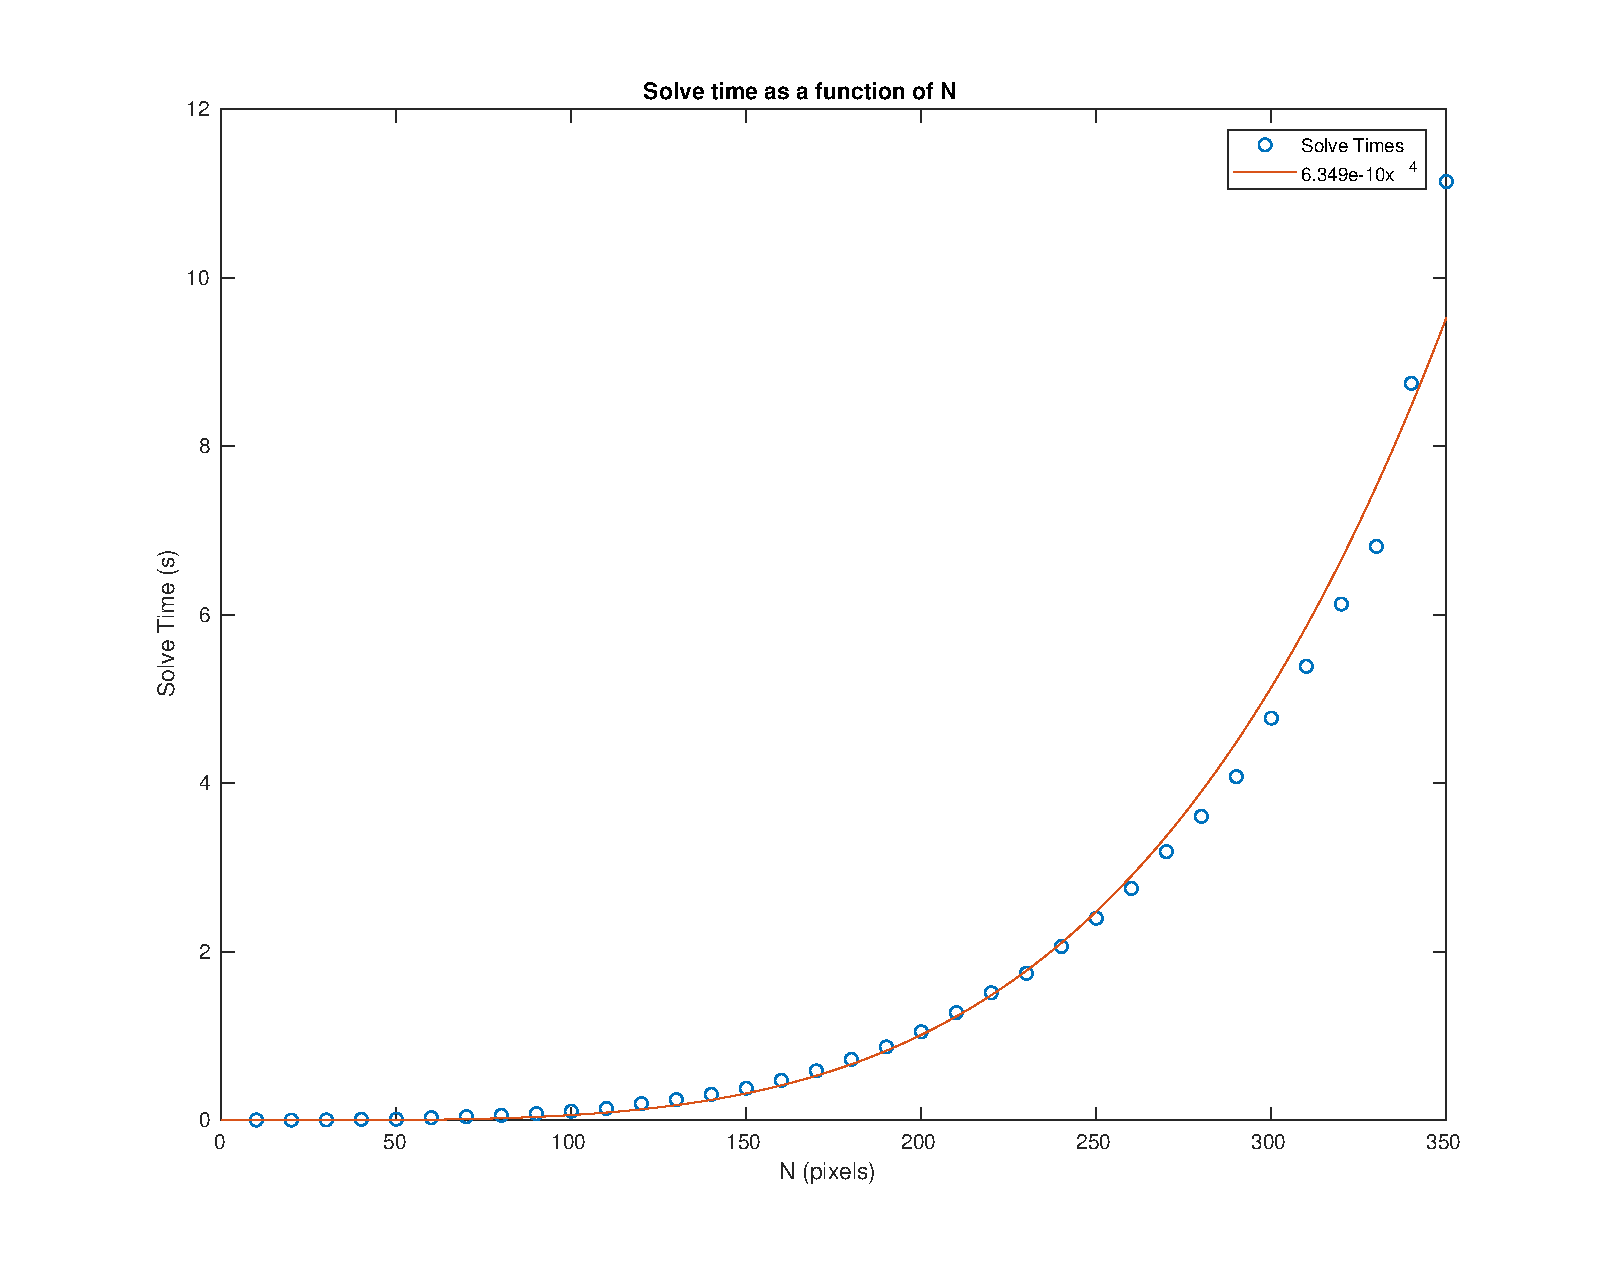
\includegraphics[scale=0.21]{sizebenchmark.eps}
	\caption{Variation of the solve time (in seconds) to $N$. The data fits
	quite well to a $N^4$ curve which is to be expected as this is the rate
	at which the matrix grows.}
	\label{sizetestFig}
\end{figure}
The code was tested with the same image at various sizes and the results were
plotted. Although exact solve times vary depending on the specific geometry,
the general trend should be the same.

Error was analysed by comparing the analytical results of Problem~0 and
Problem~1. For each pixel an absolute difference of the values was calculated
and we were able to use this to calculate the relative error of the numerical
solution.

\pagebreak
\begin{thebibliography}{9}

	\bibitem{NR}
		\emph{Numerical Recipes: The Art of Scientific Computing}\\
		W. H. Press, S. A. Teukolsky, W. T. Vetterling, B. P. Flannery\\
		September 2007\\
		ISBN: 9780521880688

	\bibitem{101matstore}
		\emph{101 Ways to Store a Sparse Matrix}\\
		Max Grossman\\
		\texttt{https://medium.com/@jmaxg3/101-ways-to-store-a-sparse
		-matrix-c7f2bf15a229}\\
		Accessed: 12\textsuperscript{th} March 2018

\end{thebibliography}



\end{document}
